\documentclass[runningheads]{llncs}

\usepackage[T1]{fontenc}
\usepackage{graphicx}
\usepackage{url}
\usepackage{cite}
\usepackage{hyperref}
\usepackage{amsmath}
\usepackage{tikz}
\usepackage{pgfplots}

\title{Development of a Mobile-Based Timeline app}

\author{Ziga Fon\inst{1} }

\institute{Univesity of Ljubljana, Faculty of Computer and Information science, Slovenia }

\maketitle
\begin{abstract}
This paper presents the development and analysis of a mobile-based timeline management application developed using React Native and Expo. The application facilitates the creation, management, and visualization of timelines with multimedia integration. This study explores the design principles, user interaction paradigms, and theoretical frameworks employed in the application, situating it within the broader context of interaction and information design.
\vspace{0.5cm}


 \newcommand{\keywords}[1]{\par\noindent{\small{\bf Keywords:} #1}}
\keywords{Interaction Design \and Mobile Application \and Timeline Management \and React Native \and Expo}


\end{abstract}

\section{Introduction}
The rapid advancement of mobile technologies has necessitated the development of applications that enhance user interaction and information management. This study focuses on a mobile-based timeline management tool designed to aid users in creating, managing, and visualizing timelines effectively. Grounded in the principles outlined in [1], this application integrates multimedia elements to provide a comprehensive storytelling experience.

Human-Computer Interaction (HCI) has evolved to encompass a broader range of interaction paradigms, including ubiquitous computing and pervasive technologies [2]. This evolution underscores the need for applications that are not only functional but also enhance user engagement through intuitive design and rich multimedia integration.
\section{Constructivist Learning Theory}

\subsection{Promoting Active Learning}
Constructivist Learning Theory emphasizes the active role of learners in constructing their own understanding and knowledge of the world, through experiencing things and reflecting on those experiences[3]. 

\subsection{Constructivism in the Timeline Project}
In the context of the Timeline Management Tool, this theory underpins the app's design by facilitating a user-centric approach where individuals actively create and manage their timelines. By allowing users to input personal events, attach multimedia content, and customize their timelines, the application enables users to engage in meaningful interactions that reflect their unique experiences and perspectives. This active participation encourages deeper cognitive processing and retention of information, aligning with the principles of constructivism. 
\newpage
\subsection{Acception of Diverse Learning Styles}
Furthermore, the ability to visualize timelines through various media formats supports diverse learning styles, fostering an inclusive environment where users can construct knowledge in ways that are most effective for them. The integration of interactive modals and customizable features ensures that users are not passive recipients but active constructors of their timelines, enhancing both the usability and educational value of the application. This alignment with Constructivist Learning Theory not only improves user engagement but also supports the development of personalized learning pathways through the management and visualization of personal and professional milestones.[4]



\section{Features Overview}
The application offers a comprehensive set of functionalities designed to provide a seamless user experience:

\begin{figure}[h]
    \centering
    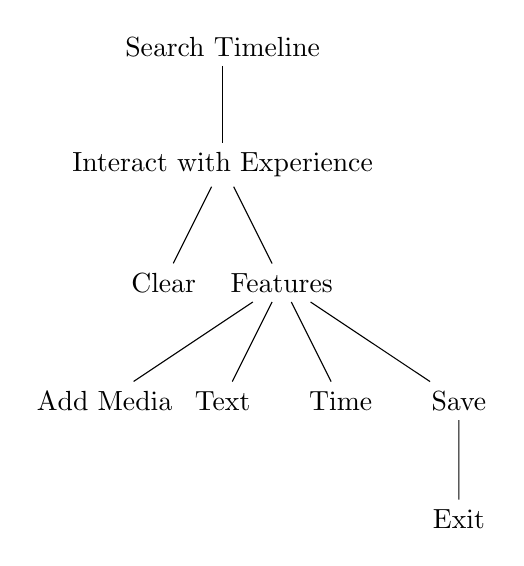
\begin{tikzpicture}
        \mindmap
        [
            grow cyclic,
            every node/.style=concept,
            concept color=orange,
            level 1/.append style={sibling angle=90},
            level 2/.append style={sibling angle=45}
        ]
        {
            \node{Search Timeline}
                child { node {Interact with Experience}
                    child { node {Clear } }
                    child { node {Features}
                        child { node {Add Media} }
                        child { node { Text} }
                        child { node { Time} }
                        child { node {Save}
                            child { node {Exit} }
                        }
                    }
                };
        }
    \end{tikzpicture}
    \caption{Typical App Usage Workflow}
    \label{fig:mindmap}
\end{figure}

\newpage


\subsection{Timeline Creation}

Users can add titles, dates, and descriptive text to define events within a timeline. The incorporation of images and videos enhances visual storytelling, enabling a richer narrative. This feature supports sequential data entry, allowing users to build timelines that reflect both personal and professional milestones.


\begin{figure}
    \centering
    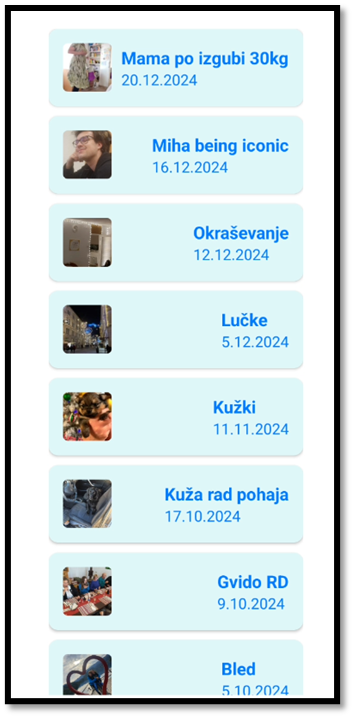
\includegraphics[width=0.55\linewidth]{image.png}
    \caption{THE TIMELINE}
    \label{fig:enter-label}
\end{figure}

\subsection{Customization}
Personalization options include adjustable background colors and dynamic organization of timeline items. The app ensures chronological sorting of events for coherent presentation. Users can select from a variety of color themes to match their aesthetic preferences, enhancing user satisfaction and engagement.

\begin{figure}
    \centering
    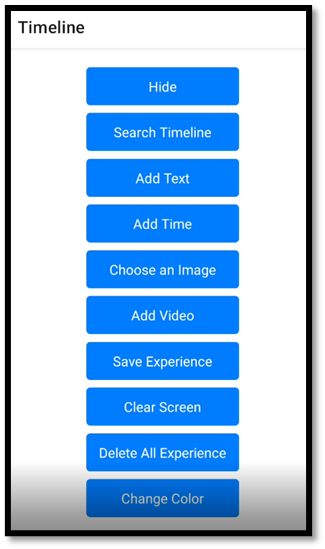
\includegraphics[width=0.6\linewidth]{image2.png}
    \caption{Costomization}
    \label{fig:enter-label}
\end{figure}


\newpage
\subsection{Media Integration}
Leveraging Expo ImagePicker and Video Player, the application allows users to import and embed multimedia content, facilitating an engaging user interface. The seamless integration of media elements ensures that timelines are not only informative but also visually appealing.


\begin{figure}
    \centering
    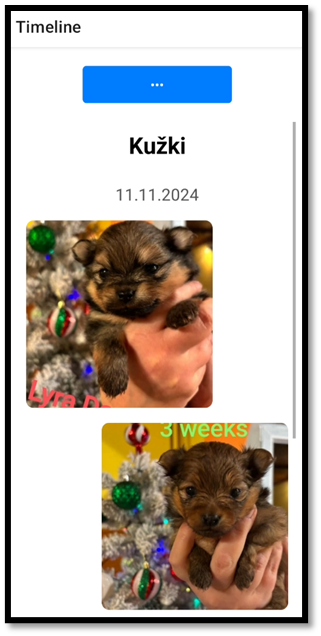
\includegraphics[width=0.55\linewidth]{image3.png}
    \caption{Timeline element Puppies}
    \label{fig:enter-label}
\end{figure}
\subsection{Storage and Retrieval}
AsyncStorage ensures persistent local storage, enabling the saving and retrieval of timelines. This feature supports data management with efficient sorting and thumbnail displays of saved events. Users can effortlessly access and modify their timelines, promoting continuous interaction with the application.

\begin{figure}
    \centering
    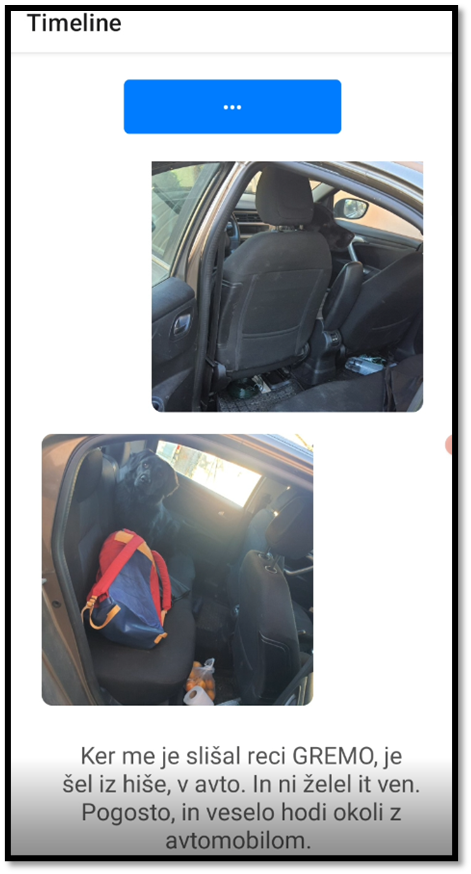
\includegraphics[width=0.5\linewidth]{image4.png}
    \caption{Example of a stored Experience in the stored Timeline}
    \label{fig:enter-label}
\end{figure}


\subsection{User Interaction}
Multiple modals facilitate adding text or time entries and browsing saved timelines. Interactive controls such as clearing timelines, deleting saved data, and toggling display options offer users a clean and guided experience. These interactions are designed to be intuitive, reducing the learning curve and enhancing usability.



\subsection{UI/UX Enhancements}
Smooth scrolling through timeline events and a clear, intuitive layout with responsive buttons and modals contribute to a positive user experience. Alert messages for success or error scenarios ensure that users are informed about the status of their actions, fostering trust and reliability in the application.

\begin{figure}
    \centering
    \includegraphics[width=0.5\linewidth]{image5.png}
    \caption{The user interface with changed color in the moment of the click}
    \label{fig:enter-label}
\end{figure}

\newpage


\section{Contextual Discussion}
Interaction design extends beyond mere usability, encompassing aspects of perception, visualization, and user engagement.

\subsection{Relation to Perception}
Understanding user perception is crucial in designing interfaces that are both intuitive and accessible. The application leverages visual hierarchy and consistent color schemes to guide user attention and facilitate information processing [5].

\subsection{Visualization Techniques}
Effective visualization techniques are employed to represent timeline data in a clear and engaging manner. The use of multimedia elements such as images and videos provides multiple modes of information representation, catering to different learning styles and preferences.


\subsection{Integration with Ubiquitous Computing}
In alignment with ubiquitous computing principles, the application is designed to be accessible across various mobile devices, ensuring that users can interact with their timelines anytime and anywhere. This flexibility supports the continuous and pervasive nature of modern user interactions.





\section{Implementation Details}
The application is built using React Native and Expo, leveraging their capabilities for cross-platform development and rapid prototyping. AsyncStorage is utilized for persistent data management, ensuring that user timelines are securely stored and easily retrievable.

\subsection{React Native and Expo}
React Native provides a robust framework for building native mobile applications using JavaScript, enabling a consistent user experience across iOS and Android platforms [6]. Expo simplifies the development process by offering a suite of tools and services that streamline testing, deployment, and scaling.

\subsection{AsyncStorage Integration}
AsyncStorage offers a simple, asynchronous key-value storage system for React Native applications. It ensures that user data, such as timelines and multimedia content, is stored persistently, allowing for offline access and reliable data retrieval [7].


\begin{thebibliography}{9}

\bibitem{preece2015interaction}
Preece, J. and Sharp, H. and Rogers, Y.
\newblock \textit{Interaction Design: Beyond Human-Computer Interaction}.
\newblock Wiley, 2015.

\bibitem{Dourish2001}
Dourish, Paul.
\newblock Seeking a foundation for context-aware computing.
\newblock \textit{Human–Computer Interaction}, 16(2--4):229--241, 2001.
\newblock \url{https://doi.org/10.1207/S15327051HCI16234_07}.

\bibitem{EdTech2025}

\newblock Constructivism in Education. 
\newblock In: EdTech Books, \textit{Student Guide}. EdTech Books, 2025. 
\newblock \url{https://edtechbooks.org/studentguide/constructivism}.



\bibitem{Smith1993}
Smith, Leslie.
\newblock \textit{Necessary Knowledge: Piagetian Perspectives on Constructivism}.
\newblock Routledge, 1st Edition, 1993. ISBN 9781138038004.
\newblock Published November 11, 2019.


\bibitem{norman2013design}
Donald A. Norman 
\newblock \textit{The Design of Everyday Things: Revised and Expanded Edition}.
\newblock MIT Press, 2013.

\bibitem{reactnative}
Facebook.
\newblock React Native Documentation.
\newblock \url{https://reactnative.dev/docs/getting-started}, 2023.

\bibitem{asyncstorage}
React Native Community.
\newblock AsyncStorage | React Native.
\newblock \url{https://reactnative.dev/docs/asyncstorage}, 2023.


\end{thebibliography}

\end{document}